\documentclass[12pt,oneside]{amsbook}
\usepackage[utf8]{inputenc}

\usepackage[
backend=bibtex,
style=alphabetic,
sorting=ynt
]{biblatex}
\addbibresource{TheBib.bib} %Imports bibliography file

\usepackage{tikz}
\usetikzlibrary{arrows}
\usepackage{graphicx}

\newtheorem{thm}{Theorem}[chapter]
\newtheorem{lemma}[thm]{Lemma}
\newtheorem{prop}[thm]{Proposition}
\newtheorem{corollary}[thm]{Corollary}

\newenvironment{defn}[1][Definition]{\begin{trivlist}
\item[\hskip \labelsep {\bfseries #1}]}{\end{trivlist}}

\newcommand{\R}{\mathbb{R}}
\newcommand{\T}{\mathcal{T}}
\newcommand{\B}{\mathbb{B}}
\newcommand{\n}{$n$}
\newcommand{\Y}{\Gamma_Y}
\newcommand{\C}{$C^2(\Y)$}


\title{Chapter 5}
\author{Tynan Daly}


\begin{document}
In the previous chapter, retracting the configuration space yielded connected discretized configuration space, however, not all spaces behave so nicely. This chapter will first examine examples of robot movement networks which do not discretize well, and then present a method for determining which graphs have a configuration space that can be discretized using a deformation retract.

\section{When Deformation Retracts are Successful}
Whenever we discretize a configuration space we eliminate portions of it, thus losing information. In the case of \C, this was a benefit as it simplified a provably safe configuration space into a more tractable one. Whenever we make a space finer, we risk losing necessary properties of our space. 

In order to demonstrate, we will discretize the two robot configuration space of the graph seen in Figure~\ref{fig:bad}, which we will call $\Gamma_{\Psi}$. Unlike $\Y$, the graph $\Gamma_{\Psi}$ contains a cycle, and so its paths need not be unique. It is these properties which will not allow us to nicely discretize its configuration space. 

\begin{figure}[h]
\centering
\caption{The Graph $\Gamma_{\Psi}$}
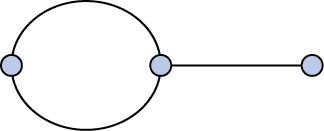
\includegraphics[scale=1]{Bad.png}
\label{fig:bad}
\end{figure}

It can be shown using a process similar to that in Chapter 3, that the configuration space for two robots on $\Gamma_{\Psi}$, denoted by $C^2(\Gamma_{\Psi})$, yields the configuration space in Figure~\ref{fig:C_Psi}.

\begin{figure}[h]
\centering
\caption{$C^2(\Gamma_{\Psi})$\cite{factory}}
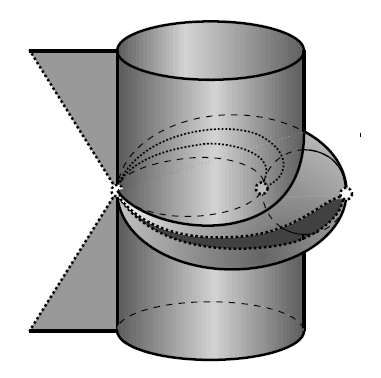
\includegraphics[scale=.5]{Bad_C.png}
\label{fig:C_Psi}
\end{figure}

Here we again see the complexity that arises when working with configuration spaces. Even though $\Gamma_{\Psi}$ seems simpler than $\Y$, its configuration space is much harder to visualize. This becomes even more apparent when we attempt to simplify $C^2(\Gamma_{\Psi})$ in order to obtain the discretized configuration space $\mathcal{D}^2(\Gamma_{\Psi})$. 

\begin{figure}[h]
\centering
\caption{$\mathcal{D}^2(\Gamma_{\Psi})$}
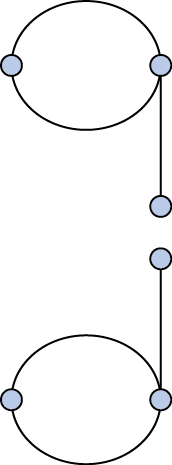
\includegraphics[scale=.5]{Bad_D.png}
\label{fig:D_Psi}
\end{figure}

The graph in Figure~\ref{fig:D_Psi} is the discretized configuration space $\mathcal{D}^2(\Gamma_{\Psi})$. Unlike $\mathcal{D}^2(\Y)$, this space cannot be used to simplify robot movement schedules. Since $\mathcal{D}^2(\Gamma_{\Psi})$ is not connected, half of the possible position configurations will be excluded depending on the initial configuration of the two robots. This renders algorithms used to find optimal movement schemes useless. 

While we can easily obtain the discretized configuration spaces for the relatively simple configuration spaces of \C and $C^2(\Gamma_{\Psi})$ by visually discretizing, this may not be the case for more complicated movement networks. The previous chapter illustrated a method for generally discretizing a configuration space by demonstrating a deformation retract on \C. In order for a space to be nicely discretizable by a deformation retract, it must meet the conditions of Theorem~\ref{thm:when}

\begin{thm}\label{thm:when}
For any $N$ robots with $N>1$, on a graph $\Gamma$ with at least $N$ vertices, $C^N(\Gamma)$ retracts onto $D^N(\Gamma)$ if and only if 

\begin{enumerate}
\item Each path between distinct essential vertices passes through at least $N-1$ edges; and,
\item Each cycle not homotopic to a point passes through at least $N+1$ edges.\cite{factory}
\end{enumerate}
\end{thm}

We know that $\Gamma_{\Psi}$ contains a cycle. Since the cycle consists of two attached $1$-cells, it cannot be retracted to a point for the same reason a closed $2$-cell cannot be retracted onto its boundary. Thus $C^2(\Gamma_{\Psi})$ cannot be nicely discretized because the cycle which is not homotopic to a point passes through only two edges and hence does not satisfy condition 2 of Theorem~\ref{thm:when}.

Discretizing \C yields a CW complex of dimension one, which we know is a graph from Chapter 3. As a result, algorithms from graph theory can be used to find optimal series of configurations for two robots to navigate a graph. We have shown that $\Y$ discretizes to a CW complex of dimension one, but we can extend this to all graphs which have radial vertices connecting a central vertex. Explicitly, we say $\Y = \Upsilon_3$, where $\Upsilon_N$ is a graph of $N-1$ vertices which are only adjacent to a central vertex. Thus every movement network belonging to $\Upsilon_N$ will discretize to a one-dimensional CW complex. Additionally, the following theorem states the the maximum dimension of the discretized configuration space is dependant on the number of vertices with degree greater than two in the movement network.

\begin{thm} \label{thm:dim}
Given a graph $G$ with $V$ vertices of degree greater than two, the discretization of $C^N(G)$ has a dimension of at most $V$.~\cite{factory}
\end{thm}

Abrams and Ghrist also show that by incorporating Theorem~\ref{thm:dim}, one can control the dimension, and therefore computational complexity, of the discretized configuration space\cite{factory}. This theorem deserves note because it allows robotic engineers to design movement schemes with the dimension of the discretized configuration space in mind. Thus we can know how to construct discretizable movement networks, build their configuration spaces, and then retract them to form their discretized forms.

Together, Theorems~\ref{thm:when} and~\ref{thm:dim} allow robotic engineers to design movement networks which will always discretize nicely while controlling for their complexity. As a result, the configuration and discretized configuration spaces of fixed movement networks such as $\Gamma_{\Psi}$ need not need to even be computed. 

\section{Conclusions}
By carefully exploring the discretization of \C, we have demonstrated how the application of topological tools can radically simplify the problem of robotic movement along fixed pathways. Beyond this explicit example however, we hope that readers view this work as guide to solving future problems pertaining to fixed path movement. 

While we feel this thesis provides a thorough examination of \C 's discretization process, work could further still be done. While we have provided a plausible method for deformation retracting \C onto $\mathcal{D}^2(\Y)$, time has unfortunately left us unable to provide a formal proof for our technique. It is our hope that the deformation retract presented in this paper could be rigorously proven in order to further illustrate discretization techniques. 

Additionally, Abrams points out in his thesis that his proof of \C 's discretization requires further work, because it incorporated Whitehead's theorem, and so we as not completely self contained\cite{thesis}. In the article he coauthored with Ghrist, however, he not only seems to solve this problem, but strengthen his theorem\cite{factory}. Exactly Abrams and Ghrist manage to strengthen their proofs merits examination which may shed further light on the mechanics involved in Theorems~\ref{thm:when} and \ref{thm:dim}.

The work done here only serves to set up the problem of robotic movement. The impetus for discretizing configuration spaces is that we may apply the tools of graph algorithms to achieve specific robot configurations. We hope that readers use this thesis as an accessible introduction to the topic so that further advancement in the field may occur.



\end{document}